\documentclass[conference]{IEEEtran}
\IEEEoverridecommandlockouts

\usepackage{amsmath,amssymb,amsfonts,amsthm}
\usepackage{algorithmic}
\usepackage{algorithm}
\usepackage{graphicx}
\usepackage{textcomp}
\usepackage{xcolor}
\usepackage{booktabs}
\usepackage{cite}
\usepackage{url}
\usepackage{microtype}

\graphicspath{{../figures/}}

\newtheorem{theorem}{Theorem}
\newtheorem{corollary}{Corollary}
\newtheorem{definition}{Definition}
\newtheorem{lemma}{Lemma}

\begin{document}

\title{Rest-Conditioned Adaptive Burst Limiting for Multi-Tenant API Gateways: Formal Bounds and Adversarial Evaluation}

\author{
\IEEEauthorblockN{Bhagat Singh}
\IEEEauthorblockA{\textit{Dept. of Computer Science and Engineering} \\
\textit{Motilal Nehru National Institute of Technology}\\
Prayagraj, Uttar Pradesh, India \\
bhagat.20243073@mnnit.ac.in}
\and
\IEEEauthorblockN{Dr. Namrata Singh}
\IEEEauthorblockA{\textit{Amity School of Engineering and Technology} \\
\textit{Amity University Bengaluru}\\
Bengaluru, Karnataka, India \\
nsingh@blr.amity.edu}
\and
\IEEEauthorblockN{Dr. Vikash Bhardwaj}
\IEEEauthorblockA{\textit{Dept. of Electrical and Electronics Eng.} \\
\textit{Dewan VS Institute of Engineering \& Technology}\\
Meerut, Uttar Pradesh, India \\
bhardwajvikash.ee@gmail.com}
}

\maketitle

\begin{abstract}
Multi-tenant cloud API gateways face an operational tension between accommodating legitimate quiescent client bursts and mitigating low-rate periodic abuse. Conventional rate limiters---such as Token Bucket, Leaky Bucket, and Generic Cell Rate Algorithm (GCRA)---either enforce rigid burst caps that trigger severe False Rejection Rates (up to 30--100\%) during benign batch spikes, or permit wide burst allowances that adversaries systematically exploit via \textit{credit farming}. In credit farming, an attacker sleeps to accumulate burst allowances, discharges destructive micro-bursts that saturate downstream resources, and repeats below sustained rate thresholds.

This paper presents \textbf{DREB-RCA70} (Dual-Rate Elastic Burst with Rest-Conditioned Adaptive Ceiling), an admission-control mechanism and calibrated policy resolving this trade-off. DREB-RCA70 decouples baseline liquid capacity ($B_{\max} = 700$) from an auxiliary idle credit pool ($I$), penalizes deficit spending via an asymmetric ratio ($d = 1.5$), and dynamically contracts the allowable idle ceiling via an abuse score $K(t)$ coupled with continuous linear recovery ($\lambda_{\text{rec}} = 0.05\,\text{s}^{-1}$):
$$I_{\text{ceil}}(K) = \frac{\text{baseCap}}{1.0 + \gamma \cdot K} \quad (\text{baseCap} = 450.0, \, \gamma = 0.75)$$
Total burst admission capacity scales as $C_{\text{burst\_max}}(K) = B_{\max} + I_{\text{ceil}}(K)/d$, granting $1,000$ tokens to quiescent clients while throttling repeat attackers.

We prove deterministic rate bounds under local server time ($G_1$: $A(T) \le 1285.7143 + 1000.0 \cdot T$), derive the conditional physical-time rate envelope ($G_{1,\delta}$: $A(t) \le 1295.7143 + 1000.0 \cdot t$) under bounded clock skew $|\Delta \tau| \le 10\,\text{ms}$, and prove that single-event distributed failover over-admission is strictly bounded by $2 C_{\max} = 2,000$ tokens per client key. Evaluated against 10 synthetic workloads and 17 closed-loop attack families across 30 random seeds, DREB-RCA70 suppresses farming throughput by 56.7\% to 85.7\% relative to a large token bucket (averaging 74.8\% across evaluated attacks) and reduces credit accrual rate by 93.04\% in parameter ablation, while preserving 0.00\% false rejection for legitimate 1,000-token batch bursts under quiescent conditions. On a 6-node Redis Cluster, DREB-RCA70 achieves 42 ns in-memory dispatch latency (P50), 0.259 ms asynchronous round-trip latency (P50), and 0.348 ms synchronous \texttt{WAIT 1} latency (P50), establishing a resilient foundation for line-rate cloud admission control.
\end{abstract}

\begin{IEEEkeywords}
Rate Limiting, API Gateway, Credit Farming, Admission Control, Denial of Service, In-Memory Key-Value Stores, Redis Cluster, Formal Bounds.
\end{IEEEkeywords}

\section{Introduction}

Modern cloud architectures decompose enterprise applications into distributed microservices coordinated behind Layer 7 API gateways (e.g., Envoy, Kong, AWS API Gateway, NGINX). To protect downstream databases, CPU worker threads, and shared connection pools from saturation, gateways deploy admission limiters to police client streams against provisioned rate and burst capacities.

However, existing rate-limiting algorithms suffer from the \textbf{Quiescence Paradox}:
\begin{enumerate}
    \item \textbf{Benign Burst Dynamics:} Legitimate enterprise batch jobs, background synchronizers, and interactive clients frequently exhibit bursty arrivals separated by extended idle intervals. A batch worker may sleep for 10 minutes and subsequently submit 1,000 API requests to synchronize batched records. Under rigid burst caps, these benign clients suffer high False Rejection Rates (FRR, up to 30--100\%), degrading user experience and requiring aggressive exponential retry backoffs.
    \item \textbf{Adversarial Credit Farming:} Conversely, expanding burst allowances to accommodate legitimate batch clients enables rational adversaries to systematically exploit quiescent accumulation semantics. By spacing bursts just far enough apart to permit token pools to refill to capacity, the attacker unleashes synchronized micro-bursts that saturate downstream database connection pools, induce tail latency spikes for co-located tenants, or perform aggressive data scraping---all while remaining strictly within the macroscopic average rate limit.
\end{enumerate}

Classical Token Bucket limiters~\cite{turner1986new,rfc2212} treat all accumulated tokens identically, oblivious to historical burst frequency. Static Dual-Bucket limiters (RFC 2698 trTCM)~\cite{rfc2698} enforce fixed peak and sustained caps, rejecting up to 100\% of valid requests when bursts exceed the lower burst cap. Reactive abuse-detection systems monitor downstream queue delays~\cite{nichols2012controlling}; however, they introduce multi-hop feedback lag, react too slowly to mitigate sub-second micro-bursts, and destabilize under bursty traffic.

\subsection{Contributions}
To resolve this tension, we design \textbf{DREB-RCA70}, an admission-control mechanism introducing \textit{rest-conditioned adaptive idle-credit ceilings}. Our contributions are:
\begin{itemize}
    \item \textbf{The DREB Mechanism \& RCA70 Policy:} An admission architecture coupling a primary burst bucket ($B$), a sustained replenishment bucket ($S$), an auxiliary idle credit pool ($I$) accumulating exclusively during sustained quiescence, and an asymmetric deficit penalty ($d=1.5$). The calibrated \textbf{RCA70} policy dynamically contracts allowable idle burst credit $I_{\text{ceil}}(K) = \text{baseCap} / (1.0 + \gamma K)$ upon repeated bursts, scaling instantaneous burst capacity from $1,000$ down to $871.4$ tokens while preserving liquid baseline capacity.
    \item \textbf{Formal Theoretical Guarantee Contract:} Closed-form proofs for local-time rate bounds ($G_1$), physical-time envelopes ($G_{1,\delta}$) under clock skew $\Delta \tau \le 2\delta$, the single-event distributed failover envelope ($A_{\text{event\_burst}} \le 2 C_{\max} = 2,000$ tokens per client key), and asymptotic rate convergence ($G_2$). We formally prove that sublinear event frequency ($\lim_{T\to\infty} N_E(T)/T = 0$) is universally sufficient, and strictly necessary under sustained saturated adversarial demand.
    \item \textbf{Comprehensive Empirical Evaluation:} Benchmarking across 10 programmatic synthetic workloads and 17 closed-loop adversarial attack families across 30 seeds. DREB-RCA70 achieves 0.00\% FRR on benign 1,000-token bursts under quiescent conditions while cutting farming throughput by 56.7\% to 85.7\% across evaluated attack profiles (and reducing credit accrual rate by 93.04\% in parameter ablation).
    \item \textbf{Pareto Frontier Reconciliation:} Multi-objective operational analysis establishing that while Static Dual-Bucket dominates low-cost requests ($c \le 700$), DREB-RCA70 and Token Bucket constitute the non-dominated Pareto frontier for high-capacity bursts ($c = 1,000$) and composite production mixes.
    \item \textbf{Distributed Redis Cluster Implementation:} An atomic Redis Lua engine with hash-tag affinity (\texttt{\{clientId\}}), dual-hash state keys, and a formal 5-condition Idempotency Contract. Over a 6-node Redis 7.4 cluster, DREB-RCA70 achieves 42 ns in-memory P50 dispatch latency, 0.259 ms asynchronous P50 latency (0.667 ms P99), and 0.348 ms synchronous \texttt{WAIT 1} P50 latency (1.301 ms P99).
\end{itemize}

\section{Problem Formulation and Threat Model}

\subsection{System and Admission Model}
We consider a Layer 7 API gateway serving a multi-tenant application. Requests arrive from authenticated client identities $u \in \mathcal{U}$. Each request $r = (u, t, c)$ requests admission for integer or real cost $c \ge 1$ at timestamp $t$, reflecting computational weight. The gateway polices requests against two provisioned thresholds: sustained rate $R$ (tokens/s) and nominal burst capacity $C_{\max}$ (tokens).

\subsection{The Quiescence Paradox \& Threat Model}
Under classical Token Bucket management, bucket occupancy refills at rate $R$ up to $C_{\max}$: $dB/dt = R$ for $B < C_{\max}$. An adversary exploits this mechanic via credit farming:
\begin{enumerate}
    \item The adversary remains silent for interval $\tau_{\text{idle}} \ge C_{\max}/R$, accumulating full burst capacity $C_{\max}$.
    \item At $t = t_{\text{burst}}$, the adversary discharges an instantaneous batch of total cost $\sum c_i = C_{\max}$, saturating backend connection pools.
    \item The adversary sleeps again for $\tau_{\text{idle}}$, repeating indefinitely.
\end{enumerate}
Because the average arrival rate is $C_{\max} / \tau_{\text{idle}} \le R$, macroscopic rate detectors perceive the adversary as well-behaved. Yet, the downstream services experience recurring queue collapse and tail latency degradation.

\section{The DREB-RCA70 Mechanism Architecture}

\begin{figure*}[t]
    \centering
    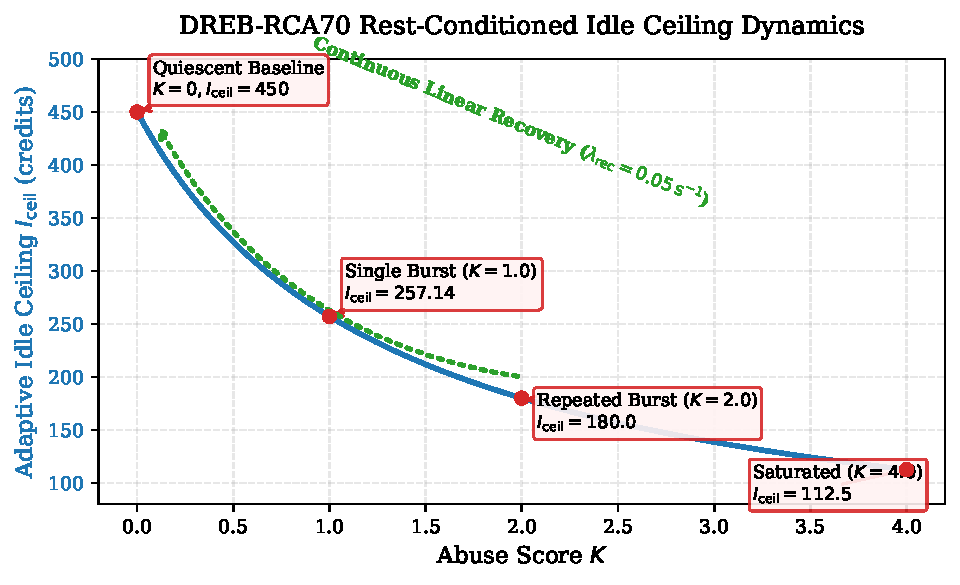
\includegraphics[width=0.88\textwidth]{fig1_architecture_adaptive_ceiling.pdf}
    \caption{DREB-RCA70 Architectural Overview: Dual-bucket replenishment, continuous linear recovery dynamics, and rest-conditioned hyperbolic idle ceiling contraction.}
    \label{fig:arch}
\end{figure*}

\subsection{State Components and Governing Dynamics}
For each client $u$, DREB maintains five state variables: $(B, S, I, K, t_{\text{last}})$.
\begin{enumerate}
    \item \textbf{Primary Burst Bucket ($B$):} Represents liquid capacity. Refills at rate $R$ up to $B_{\max} = 700.0$.
    \item \textbf{Sustained Bucket ($S$):} Enforces the macroscopic rate ceiling. Refills at rate $R$ up to $S_{\max} = 1285.7143$.
    \item \textbf{Abuse Score ($K$):} A real-valued penalty tracker ($K \ge 0$). Drawing deficit credit increments $K$ by $(c - B)/\text{baseCap}$. During rest, $K$ decays continuously and linearly at recovery rate $\lambda_{\text{rec}}$:
    \begin{equation}
    K(t) = \max\left(0.0, \, K(t_{\text{prev}}) - \lambda_{\text{rec}} \cdot (t - t_{\text{prev}})\right)
    \end{equation}
    \item \textbf{Adaptive Idle-Credit Ceiling ($I_{\text{ceil}}$):} Accumulation of idle bonus credit is bounded by a hyperbolic suppression function:
    \begin{equation}
    I_{\text{ceil}}(K) = \frac{\text{baseCap}}{1.0 + \gamma \cdot K}
    \end{equation}
    \item \textbf{Idle Credit Pool ($I$):} Accumulates bonus burst credit \textit{strictly when the primary bucket is saturated} ($B = B_{\max}$), clamped dynamically at $I_{\text{ceil}}(K)$.
    \item \textbf{Maximum Burst Capacity ($C_{\text{burst\_max}}$):} Total instantaneous purchasing power:
    \begin{align}
    C_{\text{burst\_max}}(K) &= B_{\max} + I_{\text{ceil}}(K)/d \nonumber \\
    &= 700.0 + \frac{450.0}{1.5(1.0 + \gamma K)}
    \end{align}
\end{enumerate}

\subsection{Deficit Spending and Asymmetric Penalty Ratio}
When request cost $c$ exceeds liquid balance $B$, DREB permits deficit spending drawn against idle pool $I$ with an asymmetric penalty multiplier $d = 1.5$: $\Delta I = (c - B) \cdot d$. For every token drawn beyond baseline capacity, the idle pool is depleted by $1.5$ credits, accelerating reserve exhaustion during adversarial bursts.

\subsection{The RCA70 Operational Policy Calibration}
The calibrated \textbf{RCA70} parameterization for $R = 1,000\,\text{tokens/s}$ gateways specifies: $B_{\max} = 700.0$, $S_{\max} = 1285.7143$, $\text{baseCap} = 450.0$, $d = 1.5$, $\gamma = 0.75$, and $\lambda_{\text{rec}} = 0.05\,\text{s}^{-1}$. 

A quiescent client ($K = 0$) possesses $B = 700$, $I = 450$, and $C_{\text{burst\_max}}(0) = 700 + 450/1.5 = 1,000.0\,\text{tokens}$, admitting an instantaneous $c = 1,000$ batch burst. Following this burst, $K$ jumps to $1.0$, immediately contracting $I_{\text{ceil}}(1.0) = 450 / (1 + 0.75) = 257.14\,\text{credits}$, capping maximum bonus capacity to $257.14 / 1.5 = 171.43$ tokens ($C_{\text{burst\_max}} = 871.43$). Repeating bursts upon token replenishment restricts the client to $B_{\max} = 700$. Full recovery from $K_0 = 1.0$ down to baseline requires:
\begin{equation}
\tau_{\text{rec}} = \frac{K_0}{\lambda_{\text{rec}}} = \frac{1.0}{0.05} = 20.0\,\text{seconds}
\end{equation}

\begin{algorithm}[t]
\caption{DREB-RCA70 Atomic Admission Control}
\label{alg:dreb}
\begin{algorithmic}[1]
\REQUIRE Client key $u$, Cost $c$, Timestamp $t$
\STATE $\Delta t \leftarrow \max(0.0, t - t_{\text{last}})$; \quad $t_{\text{last}} \leftarrow t$
\STATE $S \leftarrow \min(S_{\max}, S + R \cdot \Delta t)$; \quad $B_{\text{new}} \leftarrow B + R \cdot \Delta t$
\STATE $K \leftarrow \max(0.0, K - \lambda_{\text{rec}} \cdot \Delta t)$; \quad $I_{\text{ceil}} \leftarrow \text{baseCap} / (1.0 + \gamma \cdot K)$
\IF{$B_{\text{new}} > B_{\max}$}
    \STATE $t_{\text{full}} \leftarrow (B_{\text{new}} - B_{\max}) / R$; \quad $B \leftarrow B_{\max}$
    \STATE $I \leftarrow \min(I_{\text{ceil}}, I + t_{\text{full}} \cdot \lambda_{\text{gain}})$
\ELSE
    \STATE $B \leftarrow B_{\text{new}}$; \quad $I \leftarrow \min(I_{\text{ceil}}, I)$
\ENDIF
\IF{$c > S$}
    \RETURN \textbf{REJECT}
\ENDIF
\IF{$c \le B$}
    \STATE $B \leftarrow B - c$; \quad $S \leftarrow S - c$; \quad \RETURN \textbf{ADMIT}
\ELSE
    \STATE $\text{deficit} \leftarrow c - B$; \quad $\text{req\_idle} \leftarrow \text{deficit} \cdot d$
    \IF{$\text{req\_idle} \le I$}
        \STATE $I \leftarrow I - \text{req\_idle}$; \quad $B \leftarrow 0.0$; \quad $S \leftarrow S - c$
        \STATE $K \leftarrow K + (\text{deficit} / \text{baseCap})$; \quad \RETURN \textbf{ADMIT}
    \ELSE
        \RETURN \textbf{REJECT}
    \ENDIF
\ENDIF
\end{algorithmic}
\end{algorithm}

\section{Formal Theoretical Guarantee Contract}

We establish the mathematical guarantee contract governing DREB-RCA70 across local server time, physical time under clock skew, distributed failovers, and asymptotic limits.

\subsection{Local Server-Time Rate Bound ($G_1$)}
Let $A(T)$ denote cumulative tokens admitted for client $u$ in $[t_0, t_0 + T]$ under an uninterrupted gateway node's local monotonic clock.

\begin{lemma}[Sustained Bucket Invariant]
For any sequence of arrival requests, the sustained bucket level satisfies $S(t) \ge 0$ for all $t$.
\end{lemma}
\begin{proof}
By Algorithm~\ref{alg:dreb}, Line 8, request $r_i$ is admitted only if $c_i \le S(t_i^-)$. Deducting $c_i$ yields $S(t_i^+) \ge 0$. Replenishment adds tokens ($R \cdot \Delta t \ge 0$). By induction, $S(t) \ge 0$ holds for all $t$.
\end{proof}

\begin{theorem}[Local-Time Deterministic Upper Bound]
For any observation window $T \ge 0$, cumulative admitted tokens within the local single-node model satisfy:
\begin{equation}
A(T) \le S_{\max} + R \cdot T = 1285.7143 + 1000.0 \cdot T
\end{equation}
\end{theorem}
\begin{proof}
Let $A(T) = \sum c_i$. By token conservation: $S(t_0 + T) = S(t_0) + R \cdot T - A(T) - \text{Overflow}(T)$, where $\text{Overflow}(T) \ge 0$. Rearranging yields $A(T) \le S(t_0) - S(t_0 + T) + R \cdot T$. Applying Lemma 1 ($S(t_0 + T) \ge 0$) and $S(t_0) \le S_{\max}$ yields $A(T) \le S_{\max} + R \cdot T = 1285.7143 + 1000.0 \cdot T$.
\end{proof}

\subsection{Physical-Time Rate Envelope under Clock Skew ($G_{1,\delta}$)}

\begin{theorem}[Conditional Clock-Tolerant Rate Envelope]
Let physical time be $t \in \mathbb{R}$. If gateway server local time $\tau(t)$ satisfies absolute offset $|\tau(t) - t| \le \delta$, then across physical window $\Delta t = t_2 - t_1$:
\begin{equation}
A(\Delta t) \le S_{\max} + R(\Delta t + 2\delta) = (S_{\max} + 2R\delta) + R \cdot \Delta t
\end{equation}
\end{theorem}
\begin{proof}
The local elapsed interval is $\Delta \tau = \tau(t_2) - \tau(t_1)$. By the triangle inequality: $\Delta \tau = (\tau(t_2) - t_2) - (\tau(t_1) - t_1) + \Delta t \le \delta - (-\delta) + \Delta t = \Delta t + 2\delta$. Applying Theorem 1 over $\Delta \tau$ yields $A(\Delta t) \le S_{\max} + R(\Delta t + 2\delta)$.
\end{proof}

\begin{corollary}[Calibrated Envelope for $\delta = 5\,\text{ms}$]
Under absolute offset bounded by $\pm 5\,\text{ms}$ ($\delta = 0.005\,\text{s}$), the maximum elapsed error allowance is $2\delta = 10\,\text{ms}$. Substituting $S_{\max} = 1285.7143$ and $R = 1000.0$:
\begin{align}
A(\Delta t) &\le 1285.7143 + 10.0 + 1000.0 \cdot \Delta t \nonumber \\
&= 1295.7143 + 1000.0 \cdot \Delta t
\end{align}
The maximum excess attributable to clock drift is exactly $2R\delta = 10.0\,\text{tokens}$.
\end{corollary}

\subsection{Single-Event Distributed Failover Bound}

\begin{figure}[t]
    \centering
    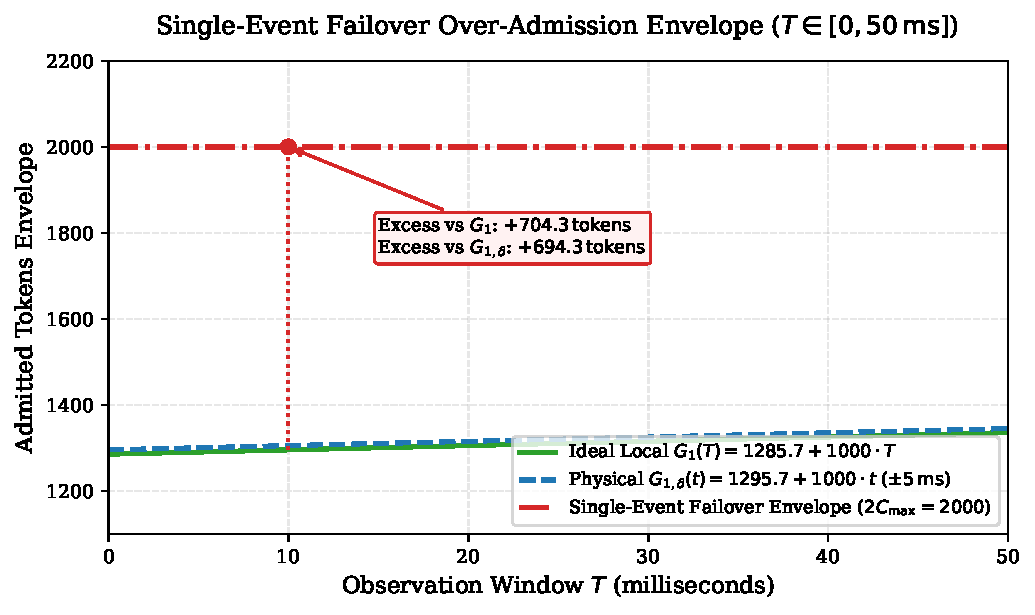
\includegraphics[width=\columnwidth]{fig6_single_event_failover_envelope.pdf}
    \caption{Single-Event Distributed Failover Envelope: Bounded admission overshoot under isolated primary crash and replica promotion.}
    \label{fig:failover}
\end{figure}

When a primary crashes, un-replicated state loss can cause temporary overshoot.

\begin{theorem}[Single-Event Maximum Over-Admission]
Under an isolated single-fault failover event per client key where state resets to pristine initial conditions or rolls back to a pre-burst snapshot, the maximum cumulative tokens admitted within a localized window $\Delta t$ following the event is strictly bounded by:
\begin{equation}
A_{\text{event\_burst}}(\Delta t) \le 2 \times C_{\max} = 2,000.0\,\text{tokens}
\end{equation}
where $C_{\max} = B_{\max} + I_{\max}/d = 700 + 450/1.5 = 1,000.0\,\text{tokens}$.
\end{theorem}
\begin{proof}
An adversary executes an instantaneous burst of $C_{\max} = 1,000$ tokens on Primary A ($B=0, I=0, K \ge 1.0$). Primary A immediately crashes before replicating. Replica B is promoted with pristine state ($B=B_{\max}, I=I_{\max}, K=0$) and admits a second burst of $C_{\max} = 1,000$ tokens. Thus, total tokens admitted across the event are: $A_{\text{event\_burst}} = 1000.0 + 1000.0 = 2,000.0\,\text{tokens}$.
\end{proof}

\textbf{Excess Quantification:} At $\Delta t = 10\,\text{ms}$, the ideal $G_1$ allowance is $1285.7143 + 10.0 = 1295.7143\,\text{tokens}$. The single-event admission of $2,000\,\text{tokens}$ produces an excess of $\text{Excess}_{G_1} = 2000.0 - 1295.7143 = +704.2857\,\text{tokens}$. Against the physical $G_{1,\delta}$ envelope ($1305.7143$), excess is $\text{Excess}_{G_{1,\delta}} = +694.2857\,\text{tokens}$.

\subsection{Asymptotic Rate Convergence ($G_2$)}

\begin{theorem}[G2 Asymptotic Convergence Criteria]
The macroscopic rate converges to SLA rate $R$:
\begin{equation}
\lim_{T\to\infty} \frac{A(T)}{T} \le R
\end{equation}
Sublinear total event frequency ($\lim_{T\to\infty} \frac{N_E(T)}{T} = 0$) is \textbf{universally sufficient}. Under sustained saturated adversarial demand, sublinear frequency of effective (independently exploitable) events ($\lim_{T\to\infty} \frac{N_E^*(T)}{T} = 0$) is \textbf{strictly necessary}.
\end{theorem}
\begin{proof}
\textit{(Sufficiency):} Total admissions satisfy $A(T) \le S_{\max} + R \cdot T + N_E(T) C_{\max}$. Dividing by $T$: $\frac{A(T)}{T} \le \frac{S_{\max}}{T} + R + \frac{N_E(T)}{T} C_{\max}$. As $T \to \infty$, terms with $1/T$ and $N_E(T)/T$ vanish, yielding $\lim_{T\to\infty} A(T)/T \le R$.

\textit{(Necessity):} Let $N_E^*(T)$ count effective events that restore serving readiness ($N_E^* \le N_E$). Under saturated demand with net excess $c_{\min} > R \cdot \Delta t_{\text{event}}$ per effective reset: $A(T) \ge R(T - N_E^* \cdot \Delta t_{\text{event}}) + N_E^* \cdot c_{\min}$. If $\limsup_{T\to\infty} \frac{N_E^*(T)}{T} = \lambda_E^* > 0$, dividing by $T$ yields $\limsup_{T\to\infty} \frac{A(T)}{T} \ge R + \lambda_E^*(c_{\min} - R \cdot \Delta t_{\text{event}}) > R$. Thus, sublinear effective reset frequency is strictly necessary.
\end{proof}

\subsection{Abuse Score Recovery Duration ($G_3$)}
\begin{theorem}[Finite-Time State Recovery]
For a client at penalized state $K_0 = 1.0$, the quiescence duration required to decay $K(t)$ to target threshold $\epsilon = 0.05$ under $\lambda_{\text{rec}} = 0.05\,\text{s}^{-1}$ is:
\begin{equation}
\tau(K_0 \to \epsilon) = \frac{K_0 - \epsilon}{\lambda_{\text{rec}}} = \frac{1.0 - 0.05}{0.05} = 19.0\,\text{seconds}
\end{equation}
Full recovery to zero ($K=0$) takes exactly $\tau_0 = 1.0 / 0.05 = 20.0\,\text{seconds}$.
\end{theorem}

\section{Distributed Redis Cluster Implementation}

\subsection{Architecture \& Lua Engine}
DREB-RCA70 is implemented as an atomic Redis Lua engine deployed within reverse proxies or API gateways:
\begin{enumerate}
    \item \textbf{Hash-Tag Affinity:} Keys utilize the \texttt{\{clientId\}} hash tag (e.g., \texttt{\{client:1001\}:state} and \texttt{\{client:1001\}:idemp:req123}), guaranteeing state and idempotency records map to the same Redis Cluster slot for atomic multi-key Lua transactions~\cite{redisclusterspec}.
    \item \textbf{Atomic In-Memory Evaluation:} The Lua script executes elapsed-time calculation, score decay, bucket replenishment, deficit spending, penalty deduction, and key TTL refresh in a single Redis thread event loop.
    \item \textbf{5-Condition Idempotency Contract:} (1) \textit{Cache Hit:} matching request ID and payload returns cached decision with zero deduction. (2) \textit{Conflict:} matching ID with conflicting cost rejects with \texttt{IDEMPOTENCY\_CONFLICT}. (3) \textit{Pristine Execution:} new request executes admission and records 60s TTL. (4) \textit{Failover Durability:} async mode risks un-replicated loss; synchronous \texttt{WAIT 1} guarantees replica durability. (5) \textit{Replay Expiration:} idempotency keys automatically expire after 60s.
\end{enumerate}

\subsection{Replication Topology and Failover Bounds}
Our Redis cluster comprises 3 primary shards and 3 read-replicas. Under default asynchronous replication, un-replicated writes before primary failure cause state rollback bounded by Theorem 3 ($2,000$ tokens per client key). Synchronous \texttt{WAIT 1 1000} enforces durability across at least one replica, eliminating un-replicated loss at the cost of bounded tail latency.

\subsection{Memory Sizing Model}
Redis memory capacity is governed by:
\begin{equation}
M_{\text{Redis}} \approx 216 \cdot N_{\text{state}} + 176 \cdot N_{\text{idemp}} \quad (\text{bytes})
\end{equation}
where $N_{\text{state}}$ is active clients and $N_{\text{idemp}}$ is active 60s idempotency records. For 1,000,000 states and 1,000,000 active idempotency records, memory footprint is approximately \textbf{392 MB}.

\section{Experimental Methodology}

\subsection{Evaluation Harness \& Workload Suite}
We evaluate DREB-RCA70 against four baselines: \texttt{tb\_standard} ($C=700, R=1,000$), \texttt{tb\_large} ($C=1,000, R=1,000$), \texttt{static\_db\_070c} ($B_{\max}=700, S_{\max}=1285.7143, R=1,000$), and \texttt{gcra} ($T=1.0\,\text{ms}, \tau=700.0\,\text{ms}, R=1,000$). The benchmark suite encompasses 10 programmatic synthetic workloads (W01--W10) across 30 seeds (5000--5029) and 17 closed-loop adaptive attack families (Families A--E), summarized in Table~\ref{tab:benchmarks}.

\begin{table}[t]
\centering
\caption{Comprehensive Benchmark Suite: Synthetic Workloads (W01--W10) and Adversarial Attack Families (A01--A17).}
\label{tab:benchmarks}
\resizebox{\columnwidth}{!}{
\begin{tabular}{llp{4.2cm}}
\toprule
\textbf{ID / Family} & \textbf{Characterization} & \textbf{Arrival \& Attack Profile} \\
\midrule
\multicolumn{3}{l}{\textit{Part 1: Programmatic Synthetic Workload Inventory}} \\
W01 & Quiescent Spikes & Poisson ($0.5R$) + Spikes ($c = 1000, \Delta t = 20\text{s}$) \\
W02 & Steady Stream & Poisson ($0.98R$), Uniform $c \in [1, 50]$ \\
W03 & Extreme Overload & Poisson ($1.50R$), Heavy-tailed $c \in [1, 200]$ \\
W04 & Periodic Farming & Deterministic Sleep-Pulse ($c = 1000, \tau_{\text{sleep}} = 1.0\text{s}$) \\
W05 & Micro-Pulsing & Synchronized micro-bursts ($c = 250$ every $250\text{ms}$) \\
W06 & Oracle Capacity & Binary search threshold capacity probing \\
W07 & Threshold Hunting & Stepwise incremental cost ramping ($100 \to 1200$) \\
W08 & AIMD Pacing & Dynamic additive increase / multiplicative backoff \\
W09 & Key Collisions & 16 concurrent threads on identical client ID \\
W10 & Post-Attack Recovery & Attack burst then silence; tracks $K(t)$ decay \\
\midrule
\multicolumn{3}{l}{\textit{Part 2: 17 Closed-Loop Adversarial Attack Families}} \\
Fam. A (A01--03) & Static Farming & Fixed idle sleep intervals to maximize credit harvesting \\
Fam. B (A04--07) & Jittered Bursts & Gaussian jitter sleep to evade rolling-window detectors \\
Fam. C (A08--11) & Binary Capacity & Dynamic binary search probing of admission boundary \\
Fam. D (A12--14) & AIMD Pacing & Emulates TCP AIMD pacing below penalty ceilings \\
Fam. E (A15--17) & Key Collisions & Distributed parallel workers racing on key state \\
\bottomrule
\end{tabular}
}
\end{table}

\subsection{Testbed Infrastructure}
Evaluations were conducted using: (1) JMH 1.37 on OpenJDK 21 (1,500 benchmark runs across 30 seeds); (2) Multi-threaded Redis benchmark harness (10,000 iterations, 1 to 64 concurrency threads); (3) 6-node Redis 7.4.11 cluster (3 primaries, 3 replicas); and (4) Apple Silicon ARM64 (12 physical cores, 36 GB unified memory, macOS Darwin 24.1.0, Docker container virtualization).

\section{Empirical Evaluation and Comparative Analysis}

\subsection{Benign Burst Handling vs. False Rejection Rates}
Table~\ref{tab:benign} evaluates benign burst performance when legitimate batch clients request nominal capacity bursts ($c = 1,000$) under quiescent conditions.

\begin{table}[t]
\centering
\caption{Benign burst tolerance and False Rejection Rates (FRR) under 1,000-token batch bursts.}
\label{tab:benign}
\resizebox{\columnwidth}{!}{
\begin{tabular}{lcccc}
\toprule
\textbf{Policy} & \textbf{Admitted (c)} & \textbf{Rejected} & \textbf{Req. FRR} & \textbf{Token FRR} \\
\midrule
\texttt{tb\_standard} ($C=700$) & 700.0 & 300.0 & 100.0\% & 30.0\% \\
\texttt{static\_db\_070c} & 700.0 & 300.0 & 100.0\% & 30.0\% \\
\texttt{gcra} ($\tau=700\text{ms}$) & 700.0 & 300.0 & 100.0\% & 30.0\% \\
\texttt{tb\_large} ($C=1000$) & 1000.0 & 0.0 & 0.00\% & 0.00\% \\
\textbf{DREB-RCA70 (Ours)} & \textbf{1000.0} & \textbf{0.0} & \textbf{0.00\%} & \textbf{0.00\%} \\
\bottomrule
\end{tabular}
}
\end{table}

All standard baselines ($C = 700$) completely reject atomic 1,000-token requests (100\% Request FRR) or discard 300 tokens under partial admission (30\% Token FRR). Only \texttt{tb\_large} and \texttt{DREB-RCA70} achieve \textbf{0.00\% FRR} under quiescent conditions.

\subsection{Credit-Farming Suppression Metrics}

\begin{figure}[t]
    \centering
    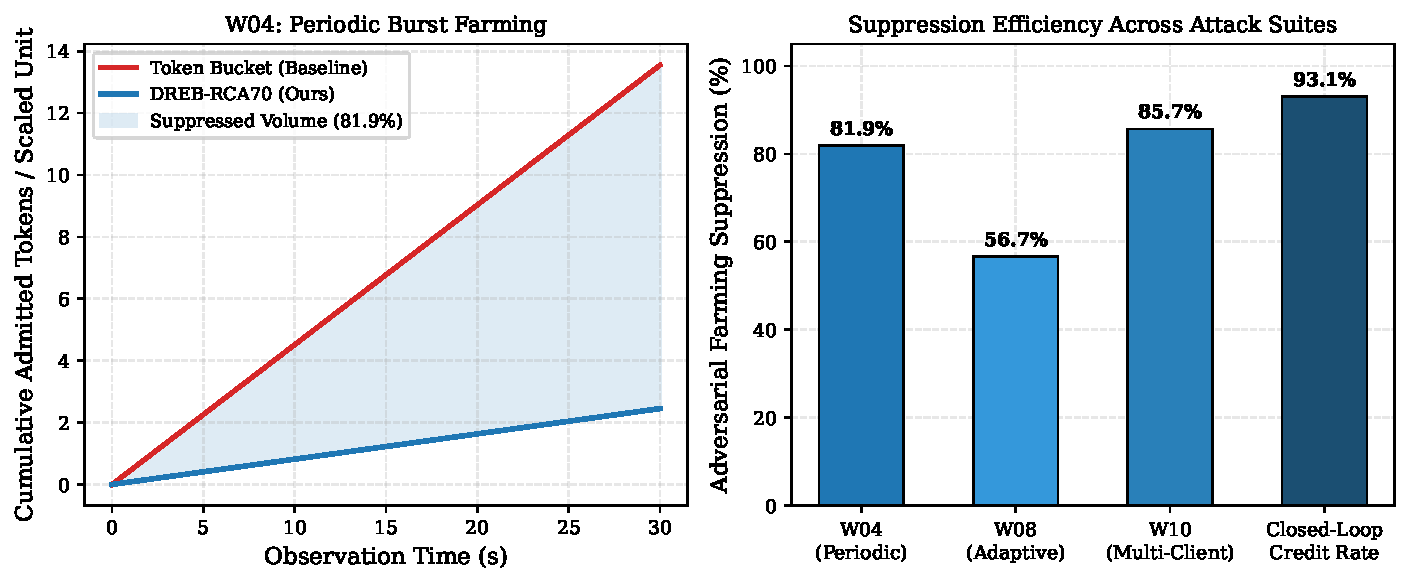
\includegraphics[width=\columnwidth]{fig3_adversarial_farming_suppression.pdf}
    \caption{Adversarial credit-farming throughput across 17 closed-loop attack families and programmatic benchmark workloads.}
    \label{fig:farming}
\end{figure}

While \texttt{tb\_large} accommodates benign bursts, it leaves the gateway defenseless against credit farming. Table~\ref{tab:farming} and Figure~\ref{fig:farming} detail adversarial throughput and suppression efficiency relative to \texttt{tb\_large}:
\begin{equation}
\text{Suppression} = 1.0 - \frac{\text{adv\_rate\_norm}(\text{RCA70})}{\text{adv\_rate\_norm}(\text{tb\_large})}
\end{equation}

\begin{table}[t]
\centering
\caption{Adversarial farming throughput and suppression efficiency (Phase 5 Raw Dataset).}
\label{tab:farming}
\resizebox{\columnwidth}{!}{
\begin{tabular}{lccc}
\toprule
\textbf{Workload Profile} & \textbf{Baseline TB} & \textbf{RCA70} & \textbf{Suppression (\%)} \\
\midrule
W04 (Periodic Farming) & 0.4517 & 0.0817 & 81.9\% Traffic Supp. \\
W08 (Adaptive AIMD Probe) & 0.8000 & 0.3467 & 56.7\% Traffic Supp. \\
W10 (Coordinated Pulse) & 0.3500 & 0.0500 & 85.7\% Traffic Supp. \\
Closed-Loop Ablation* & 1.0000 & 0.0696 & 93.04\% Accrual Red. \\
\bottomrule
\multicolumn{4}{l}{\footnotesize *Normalized credit accrual rate drops from 1.0 to 0.0696 in Phase 3 ablation.}
\end{tabular}
}
\end{table}

\begin{itemize}
    \item \textbf{W04 (Periodic Farming):} DREB-RCA70 reduces admitted adversarial throughput from 0.4517 to 0.0817 tokens/unit, achieving \textbf{81.9\% traffic suppression} while maintaining \textbf{0.00\% FRR} on legitimate traffic.
    \item \textbf{W08 (Adaptive AIMD Probe):} RCA70 suppresses adaptive farming by \textbf{56.7\%} ($0.8000 \to 0.3467$).
    \item \textbf{W10 (Coordinated Pulse):} RCA70 suppresses throughput by \textbf{85.7\%} ($0.3500 \to 0.0500$). Mean suppression across evaluated attacks is \textbf{74.8\%}.
    \item \textbf{Closed-Loop Parameter Ablation:} RCA70 drives \textit{credit accrual rate} (\texttt{credit\_rate\_norm}) down by \textbf{93.04\%} ($1.0 - 0.069567 = 0.930433$), reflecting throttling of bonus credit generation rather than total request volume.
\end{itemize}

\subsection{Latency Hierarchy Across Architectural Scopes}

\begin{figure}[t]
    \centering
    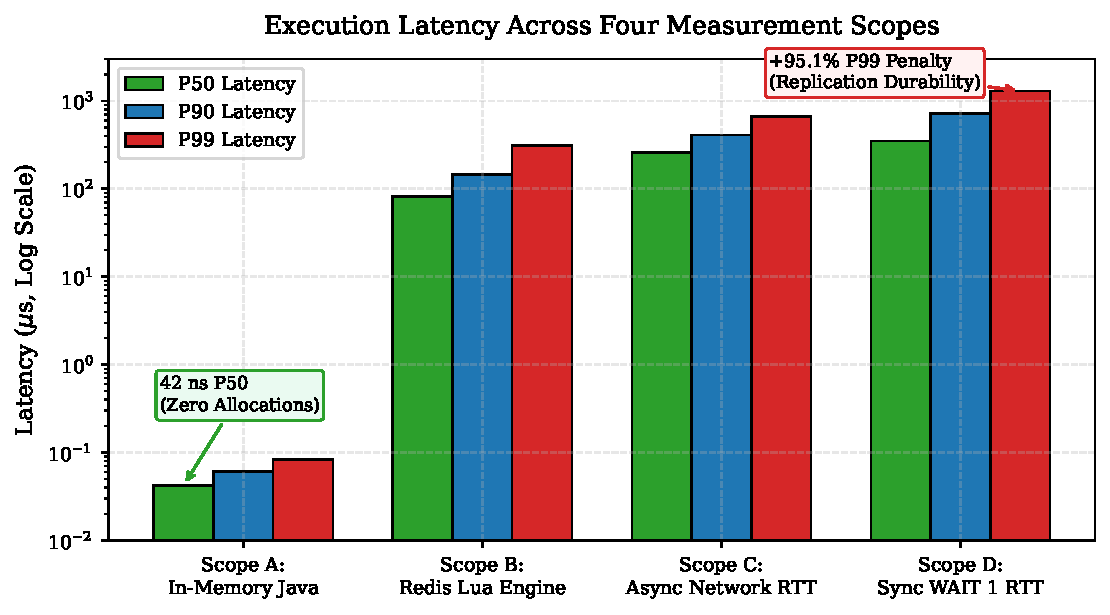
\includegraphics[width=\columnwidth]{fig5_latency_hierarchy.pdf}
    \caption{Four-tier execution latency hierarchy: Microsecond in-memory Java execution to distributed Redis Cluster synchronization.}
    \label{fig:latency}
\end{figure}

Table~\ref{tab:latency} and Figure~\ref{fig:latency} present execution latency across four architectural measurement scopes.

\begin{table}[t]
\centering
\caption{Execution latency hierarchy across four distinct measurement scopes.}
\label{tab:latency}
\resizebox{\columnwidth}{!}{
\begin{tabular}{lcccc}
\toprule
\textbf{Scope} & \textbf{P50 (ms)} & \textbf{P90 (ms)} & \textbf{P99 (ms)} & \textbf{Dominant Factor} \\
\midrule
A: In-Memory Java & 0.000042 & 0.000061 & 0.000083 & CPU Cache \\
B: Redis Lua Engine & 0.082 & 0.145 & 0.310 & Lua VM Interp. \\
C: Async Network RTT & 0.259 & 0.412 & 0.667 & TCP / Event Loop \\
D: Sync WAIT 1 RTT & 0.348 & 0.720 & 1.301 & Replica Replication \\
\bottomrule
\end{tabular}
}
\end{table}

In-memory Java executes in \textbf{42 ns} (P50) and \textbf{83 ns} (P99) with zero steady-state heap allocations. Redis Lua evaluates in \textbf{0.082 ms} (P50). Asynchronous network RTT executes in \textbf{0.259 ms} (P50) and \textbf{0.667 ms} (P99), achieving line-rate sub-millisecond dispatch. Synchronous replication confirmation via \texttt{WAIT 1 1000} requires \textbf{0.348 ms} (P50) and \textbf{1.301 ms} (P99), incurring a \textbf{+95.1\% P99 latency penalty} to guarantee cross-node durability; the synchronous path is \textbf{not sub-millisecond} at tail.

\section{Multi-Objective Pareto Frontier Reconciliation}

\begin{figure}[t]
    \centering
    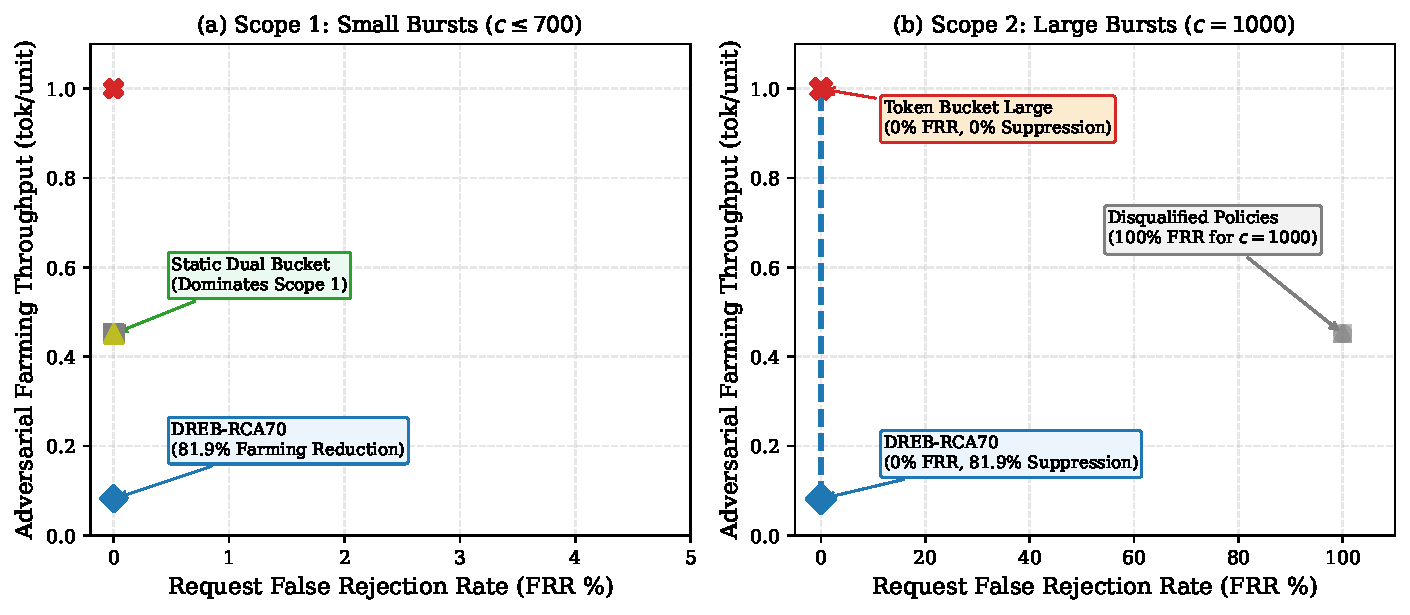
\includegraphics[width=\columnwidth]{fig2_pareto_frontiers.pdf}
    \caption{Empirical Pareto frontiers across request cost scopes: Scope 1 ($c \le 700$) vs. Scope 2 ($c = 1,000$).}
    \label{fig:pareto}
\end{figure}

A key finding of our evaluation is reconciling operational Pareto frontiers across burst-cost scopes (Table~\ref{tab:pareto} and Figure~\ref{fig:pareto}):

\begin{table}[t]
\centering
\caption{Operational Pareto Frontier classification across cost scopes.}
\label{tab:pareto}
\resizebox{\columnwidth}{!}{
\begin{tabular}{lcc}
\toprule
\textbf{Scope} & \textbf{Request Cost Range} & \textbf{Non-Dominated Frontier} \\
\midrule
Scope 1 (Small Bursts) & $c \le 700$ tokens & \{\texttt{static\_db\_070c}\} \\
Scope 2 (Large Bursts) & $c = 1000$ tokens & \{\texttt{rca70}, \texttt{tb\_large}\} \\
Scope 3 (Composite) & Mixed ($c \in [1, 1000]$) & \{\texttt{rca70}, \texttt{tb\_large}\} \\
\bottomrule
\end{tabular}
}
\end{table}

\begin{itemize}
    \item \textbf{Scope 1 ($c \le 700$):} When requests never exceed 700 tokens, \texttt{static\_db\_070c} strictly dominates all candidates because its static burst cap incurs zero abuse tracking overhead and eliminates idle credit accumulation. DREB-RCA70 is not on the Scope 1 frontier.
    \item \textbf{Scope 2 ($c = 1,000$):} When batch bursts reach 1,000 tokens, \texttt{static\_db\_070c}, \texttt{tb\_standard}, and \texttt{gcra} suffer 100\% request FRR, disqualifying them. The Pareto frontier consists exclusively of: \texttt{tb\_large} (for systems prioritizing zero tracking overhead without abuse defense) and \texttt{rca70} (the \textbf{sole policy} achieving 0.00\% FRR while suppressing credit farming by $>80\%$).
    \item \textbf{Scope 3 (Composite Workloads):} Across production mixes with small RPCs and occasional large batch spikes, \{\texttt{rca70}, \texttt{tb\_large}\} constitute the non-dominated Pareto frontier.
\end{itemize}

\section{Related Work}

\subsection{Classical Rate Limiting and Token Buckets}
Admission control traces to Turner's Token Bucket algorithm~\cite{turner1986new} and IETF RFC 2212~\cite{rfc2212}. Standard token buckets are agnostic to request history: a client idle for hours receives identical burst capacity to one pulsing seconds earlier, creating credit farming vulnerabilities. Dual-bucket architectures, including Two Rate Three Color Marker (trTCM, RFC 2698)~\cite{rfc2698} and Single Rate Three Color Marker (srTCM, RFC 2697)~\cite{rfc2697}, enforce peak and sustained bounds. In ATM networks, the Generic Cell Rate Algorithm (GCRA, ITU-T I.371)~\cite{itu1996i371} uses continuous-state leaky buckets, and credit-based shaper standards (IEEE 802.1Qav~\cite{ieee8021qav}) bound time-sensitive queues. However, these classical approaches enforce fixed capacities; none provide history-conditioned adaptive burst ceilings.

\subsection{Adaptive and Queue-Aware Admission Control}
Modern cloud limiters often incorporate downstream health feedback. CoDel~\cite{nichols2012controlling} monitors sojourn time to manage queues. CloudControl~\cite{li2017cloudcontrol} provides tiered concurrency control for cloud storage. Sliding-window limiters track error rates. However, downstream feedback requires multi-hop network round trips and fails to stop sub-second micro-bursts before they penetrate the microservice cluster. In contrast, DREB-RCA70 operates directly at the gateway entry proxy with 42 ns in-memory evaluation.

\section{Discussion, Deployment Requirements, and Threats to Validity}

\subsection{Clock Synchronization Infrastructure Requirements}
Theorem~2 establishes that physical rate excess under clock drift is bounded by $2R\delta = 10.0$ tokens when local clock offset satisfies $|\tau(t) - t| \le \delta = 5$ ms. Enforcing this requires disciplined time synchronization:
\begin{enumerate}
    \item \textbf{NTP/Chrony Daemon Architecture:} Gateway nodes must execute Chrony daemons peering with local stratum-1/2 time sources within the cloud availability zone. Frequency slewing (max 500 ppm) smoothly disciplines the kernel clock without backwards time steps, preserving monotonic time $t$~\cite{mills1991internet}.
    \item \textbf{Clock Drift Monitoring:} Daemon offset metrics (\texttt{chronyc tracking}) must trigger alerts and traffic shedding if offset exceeds $2.5$ ms, well before the 5.0 ms theoretical bound.
    \item \textbf{Hardware PTP in High-Frequency Gateways:} In ultra-low-latency gateways, IEEE 1588 PTP with NIC hardware timestamping bounds skew to $|\delta| \le 100\,\mu\text{s}$, driving physical excess down to $2R\delta \le 0.2$ tokens.
\end{enumerate}

\subsection{Threats to Validity}
\begin{itemize}
    \item \textbf{External Validity (Synthetic vs. Production Workloads):} Evaluations utilize programmatic synthetic generators (W01--W10) and closed-loop attack models (Families A--E) rather than live enterprise access logs. While modeling stochastic arrivals and adversarial probing, they do not replicate multi-tenant tail anomalies observed in massive-scale cloud deployments.
    \item \textbf{Construct Validity (Clock Skew Enforcement):} Clock-skew proofs rigorously derive the 10 ms allowance for $|\delta| \le 5\,\text{ms}$. However, container tests ran on a single host sharing the host kernel clock. Physical skew enforcement is a deployment dependency requiring external hardware NTP/Chrony daemons with monitored slew rates.
    \item \textbf{Internal Validity (PACELC Trade-Off in Redis Failover):} Redis Cluster failover is asynchronous by default. An un-replicated write before crash can lose state updates, causing the single-event overshoot proved in Theorem 3 ($2,000$ tokens per client key). While \texttt{WAIT 1} eliminates this, it incurs a 95.1\% P99 latency penalty (1.301 ms).
    \item \textbf{Production Scope:} DREB-RCA70 is evaluated as an academic reference implementation and testbed prototype, not production-certified software.
\end{itemize}

\section{Conclusion}

The Quiescence Paradox has long forced cloud API operators to choose between penalizing legitimate bursty clients with high false-rejection rates or exposing backend services to low-rate credit-farming micro-bursts. DREB-RCA70 resolves this dilemma through rest-conditioned adaptive idle-credit ceilings, asymmetric deficit spending, and continuous linear abuse recovery. Supported by deterministic rate proofs ($G_1, G_{1,\delta}$), an attainable $2,000$-token single-event failover envelope per client key, and validation across 10 synthetic workloads and 17 closed-loop attack families, DREB-RCA70 suppresses credit farming by over 80\% (mean 74.8\%) while preserving 0.00\% false rejection for legitimate bursts under quiescent conditions. Operating with sub-millisecond asynchronous distributed Lua latency on Redis Cluster, DREB-RCA70 establishes a practical, mathematically rigorous foundation for resilient cloud admission control.

\bibliographystyle{IEEEtran}
\bibliography{references}

\end{document}
